%!TEX root = skripsi.tex
%-----------------------------------------------------------------------------%
\chapter{\babDua}
%-----------------------------------------------------------------------------%
Bab ini membahas mengenai studi literatur yang digunakan selama penelitian. Studi literatur ini menjelaskan tentang hal-hal mendasar yang dibutuhkan dalam penelitian.

%-----------------------------------------------------------------------------%
\section{Word Sense Disambiguation}
%-----------------------------------------------------------------------------%
\textit{Word Sense Disambiguation} merupakan salah satu penelitian di bidang NLP yang bertujuan untuk menentukan makna yang paling tepat dari suatu kata berdasarkan konteks kata tersebut ditemukan. Sebagaimana kata dalam suatu bahasa bisa memiliki makna lebih dari satu (polisemi), \textit{task} ini akan menentukan makna kata mana yang paling tepat.

Penentuan makna kata yang tepat oleh sistem WSD ditentukan berdasarkan konteks dari kata tersebut berada. Walaupun satu kata dapat memiliki beberapa makna, terdapat kecil kemungkinan bahwa kata yang sama digunakan dalam satu \textit{discourse} untuk menyatakan makna yang berbeda sebagaimana "one sense per discourse" \citep{gale1992one}

%-----------------------------------------------------------------------------%
\section{Word Sense Induction}
%-----------------------------------------------------------------------------%	
%-----------------------------------------------------------------------------%	
\textit{Word Sense Induction} (WSI) adalah sebuah \textit{task} yang mempunyai fungsi utama untuk mendapatkan makna kata dari sebuah korpus atau teks yang belum dianotasi secara otomatis. WSI dapat dilakukan jika penelitian WSD yang ingin dilakukan tidak mempunyai cukup \textit{resource} seperti misalnya Wordnet yang memadai. Terdapat berbagai macam pendekatan dalam melakukan WSI, diantaranya adalah dengan melakukan \textit{clustering} kata \citep{denkowski2009survey}, ataupun menggunakan pendekatan \textit{cross language}.
	
	\subsection{Pendekatan \textit{Clustering}}
	Dua kata dianggap dekat secara semantik jika memiliki \textit{co-occurrence} dengan kata-kata tetangganya yang sama \citep{nasiruddin2013state}. Konsep tersebut mendasari cara WSI mendapatkan \textit{sense} kata secara implisit berdasarkan hasil \textit{cluster} yang terbentuk dari data atau teks mentah (teks yang tidak dianotasi). 
	
	\subsection{Pendekatan \textit{Cross Language}}
	Selain pendekatan \textit{clustering}, WSI juga dapat memanfaatkan fitur dimana satu kata dari suatu bahasa, dapat diterjemahkan menjadi beberapa kata di bahasa lain. Contoh kasus tersebut dapat dilihat pada kata "halaman" berikut:



	(K1-Indonesia): Aku membaca 10 \textbf{halaman} buku Harry Potter
	
	(K1-English): I read 10 \textbf{pages} of Harry Potter book
	
	(K2-Indonesia): Ani tinggal di rumah dengan \textbf{halaman} yang sangat luas
	
	(K2-English): Ani lives in a house with very large \textbf{yard}
	
	
	
	Berdasarkan kedua pasangan kalimat tersebut, kata \textbf{halaman} dalam bahasa Indonesia dapat diterjemahkan menjadi dua buah kata dalam bahasa Inggris, yaitu \textit{page} ataupun \textit{yard}. Hal ini menunjukan bahwa terjemahan dari suatu kata bergantung pada makna yang dikandung kata tersebut.

%-----------------------------------------------------------------------------%
\section{Evaluasi \textit{Word Alignment}}
Tugas dari \textit{word alignment} adalah menemukan korespondensi antara kata dan frasa pada teks paralel 
\citep{mihalcea2003evaluation}. Evaluasi ini akan membandingkan antara hasil \textit{alignment} dari sebuah tool \textit{word alignment} dengan hasil \textit{alignment} manusia sebagai \textit{gold standard}. Kasus yang dapat terjadi pada proses \textit{alignment} ini adalah ketika terdapat kata yang tidak memiliki pasangan. Contoh dari kasus tersebut dapat dilihat pada pasangan kaimat berikut:


K1(en) : \textit{He would do it regardless what people say}

K1(id) : Dia akan melakukannya segalanya


Bila melihat bahasa Indonesia sebagai sumber bahasa, maka kata "segalanya" pada kalimat tersebut tidak memiliki pasangan. Pada kasus seperti contoh diatas, kata yang tidak memiliki pasangan akan dipasangkan dengan \textit{token} NULL.


Selain kata yang tidak memiliki pasangan, terdapat juga kasus dimana pasangan adalah berupa frasa. Hal ini dapat dilihat pada contoh berikut:


K2(en) : The victim must be taken to the hospital

K2(id) : Korban tersebut harus di bawa ke rumah sakit


Berangkat dari bahasa asal yaitu Indonesia, kata "rumah sakit" dipasangkan kepada kata "hospital". Hal ini dapat berlaku berkebalikan jika bahasa asal yang digunakan adalah bahasa Inggris seperti kata "untuknya" berpasangan dengan kata "for him".

\subsection{Tokenisasi}
Pada proses evaluasi ini, pemisah kata yang umum digunakan untuk tokenisasi adalah karakter spasi. setiap token dari hasil tokenisasi tersebut kemudian dianggap sebagai satu unit kata. Kata ini akan diindeks dengan angka untuk mempermudah proses \textit{alignment} dan komputasi evaluasi. Contoh tokenisasi dan pemberian indeks pada kalimat "Aku ingin membeli mainan" adalah:

K3(id) : Aku ingin membeli mainan
K3(indeks) : 1 2 3 4

\subsection{Pengukuran Evaluasi}
Terdapat empat buah pengukuran berbeda, yaitu \textit{precision}, \textit{recall}, \textit{f-measure}, dan \textit{alignment error rate (AER)}. Diberikan hasil \textit{alignment} dari program berupa A, dan \textit{gold standard alignment} dari \textit{evaluator} (manusia) sebagai G, masing-masing mengandung dua buah \textit{set} yaitu \textit{probable alignment} dan \textit{sure alignment}. Pengukuran evaluasi dapat dilakukan dengan cara berikut:

\begin{figure}
	\centering
	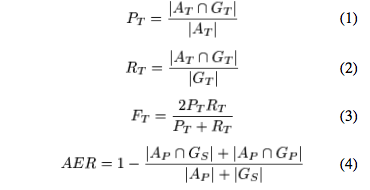
\includegraphics[width=1\linewidth]{adit_pics/Pengukuran-Word-Alignment}
	\caption{Pengukuran Word Alignment}
	\label{fig:Pengukuran-Word-Alignment}
\end{figure}
%------------------------------------------- ----------------------------------%
